% sci.tex - SCI STYLE FILE 使用例

\documentclass{ujarticle}
\usepackage{sci}
\usepackage{amsmath}
\usepackage[dvipdfmx]{graphicx}
\usepackage{bmpsize}
\usepackage{here}
% 日本語原稿の場合
% 
% LaTeX2e
% \documentclass{jarticle}
% \usepackage{sci}
% 
% LaTeX209
% \documentstyle[sci]{jarticle}

% 英語原稿の場合
% 
% LaTeX2e
% \documentclass{article}
% \usepackage{latexsym}
% \english
% 
% LaTeX209
% \documentstyle[sci]{article}
% \english

% 2006-11-16 modification by TF %SCI07

\jtitle{クラウドソースドマニュファクチャリング環境下における\\オークションに基づくリソース配分手法の提案}
\etitle{A proposal of Auction based resource allocation method under Crowdsourced Manufacturing environment}
\jauthor{○原田 佳明, 貝原 俊也, 國領 大介,,藤井 信忠(神戸大学)}
\eauthor{*Y. Harada, T. Kaihara, D. Kokuryo and N. Fujii (Kobe Univ.)}
\englishabstract{With the development of IoT technology, a production form called “Crowdsourced Manufacturing System” is attracting attention, which shares information on resources possessed by individual companies and enables their mutual use. In this paper, we propose an auction-based method that can determine resource allocation and trade prices under distributed decision-making in this paper. To verify its effectiveness.
}

\begin{document}

\maketitle

\section{はじめに}
近年IoT(Internet of Things)の発展に伴い,工場や製造機器をインターネット上に繋
ぐことにより生産性を向上させるための動きが活発化している.
また,企業や工場内だけでなく,企業の壁を超えたつながりを利用した生産形態に注目が集まっ
ている\cite{IVI}.我々は,その中でIoT 環境下において複数の工場や複数の企業をつなぎ設備・材料・
労働力・工法を融通し合う生産形態であるクラウドソースドマニュファクチャリングシス
テムに着目する\cite{IEC}.
クラウドソースドマニュファクチャリングシステムを形成することで,例えば,需要過多となりリソースが不足し
た処理を他企業に委託することで,リソース不足への対応を行うことができる.また他
企業に委託することで,近年多様化する顧客ニーズに
合わせたカスタム生産を低コストで実現可能となる.1企業で様々な機器等を
揃えるのは高コストになってしまうが,必要なときに必要なリソースをクラウドソースドマニュファ
クチャリング上から借りることにより,低コストでの生産を可能とする.また,リソースを
提供する企業は,リソースの不稼働時間を有効活用し提供料金により利益を得ることが
できる\cite{勝村}.そのためにはクラウドソースドマニュファクチャリング内の企業か
らの要求を,提供リソースを持つ企業に対して適切に割当てるリソース配分手法が重要と
なる\cite{Wu}.そこで我々は,分散された意思決定下で,財の割り当てと取引価格を
決めることのできるオークション方式に着目する.本稿では売り手と買い手の片方が入札を行い,それによ
り配分と取引価格を決めるシングルオー
クションに基づくリソース配分手法と,売り手と買い手の双方が入札を行い,それによ
り配分と取引価格を決めるダブルオークションに基づくリソース配分手法の
2つの手法を提案し,計算機実験によりその特性の評価を行う.
\section{対象モデル}
本稿の対象とするクラウドソースドマニュファクチャリングモデルの概要を
\figref{fig:CsMfg}に示す.リソースを要求する企業をリソース要求側,リソースを提供
する企業をリソース提供側とする.以下にその特徴を示す.
\begin{figure}[H]
  \centering
  \includegraphics[width=0.5\textwidth]{CsMfg.pdf} 
  \caption{Crowdsourced Manufacturing model}
  \label{fig:CsMfg}
\end{figure}
\begin{itemize}
  \item {対象とする製品は,工程毎に分割可能とする.}
  \item {各企業のリソースの管理と配分を決めるオークション主催者が存在する.}
  \item {顧客からのオーダは各企業に対して行われる.}
  \item {各企業は出来ない処理がある場合に,必要なリソースとその量をオークショ
      ン主催者に対し要求する.} 
  \item {リソース要求企業はリソースが提供されれば,製品の生産を行う.}
  \item {各企業は空いているリソースがあればオークション主催者に提示し,リソースを提供する.}
\end{itemize}
\section{オークションに基づくリソース配分手法}
リソースの要求に対して,提供リソースを割当てるためのシングルオークションに基づく
手法とダブルオークションに基づく提案手法
について説明する.以下の[Ts]はタイムスロットを示す.
\subsection{シングルオークションに基づくリソース配分手法}
シングルオークションに基づいたリソース配分手法はリソースの提供側が入札を行う.リソースの要求側は予算と要求を提示するが,こちらの予算は保障額と
してのみ使用される.
\subsubsection{全体の流れ}
\begin{description}
\item [STEP1.] {リソース提供企業は入札,リソース要求企業はリソース要求を作成し,クラウド
    オークション主催者に提出する(リソース要求と入札作成).}
\item [STEP2.] {オークション主催者は,評価値の合計が最大(最少)となる入札を決定する(勝者決定).}
\item [STEP3.] {各企業はオークションの結果に応じ,定められた取 引価格において取引を行う(取引価格決定).}
\end{description}
オークション主催者は利益を求めないとする.またオークションにかけられる財はリソー
ス$r(=1,\cdots ,R)$とする.
\subsubsection{入札とリソース要求の作成}
リソース提供企業($i=1 \cdots I$)の入札を以下で説明する.
\begin{itemize}
\item {提供するリソース$r$のコストに利益を上乗せした提供単価$p_{i,r}$と提供時間$TP_{i,r}$からなる入札を作成}
\item {$R$個の入札を作成}
\item {提供時間の一部のみを提供することが可能である}
\end{itemize}
リソース提供側の入札の例を\figref{fig:bid-provider-single}に示す.
\figref{fig:bid-provider-single}は企業1はリソース1を提供単価0.2[円]で150[Ts],リソース2
を提供単価0.4[円]で100[Ts]提供できることを示す.
\par
\begin{figure}[htb]
  \centering
  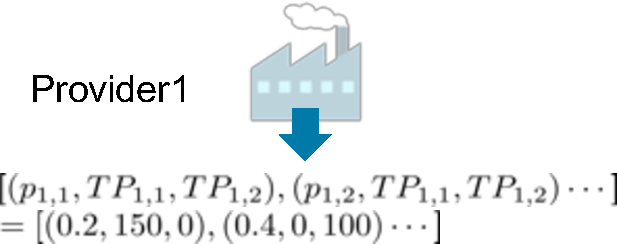
\includegraphics[width=0.35\textwidth]{bid-provider-single.pdf} 
  \caption{Bid of provider in single auction}
  \label{fig:bid-provider-single}
\end{figure}
リソース要求側($\j=1 \cdots J$)のリソース要求について説明する.リソース要求側は予算とリソース要求を提示する.この予算は保証額にのみ使用され,取引価格や
配分には使用されない.以下で作成される要求について説明する.
\begin{itemize}
\item {リソース要求$n$,予算$v_{n,j}$要求するリソース$r$の要求時間$TR_{j,n,r}$を提示する} 
\item {各企業は$N$個のリソース要求を作成}
  \begin{itemize}
  \item {ただし$N$個のリソース要求のうち勝者となる要求は1つ} 
  \end{itemize}
\item {必要なリソースの組合せに対してリソースの要求を作成する}
    \begin{itemize}
    \item {全てのリソースが揃わないと製品の生産が出来ないからである}
    \item {1つの要求内のリソースはある1提供企業によって提供されるとする}
    \end{itemize}
\end{itemize}
作成されるリソース要求の例を\figref{fig:request}に示す.\figref{fig:request}はリソース要
求企業1は予算150[円]でリソース1を150[Ts],リソース2を50[Ts]要求することを示す.
\begin{figure}[htb]
  \centering
  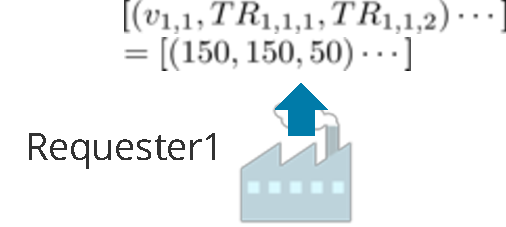
\includegraphics[width=0.3\textwidth]{bid-requester.pdf} 
  \caption{Request in single auction}
  \label{fig:request}
\end{figure}
\subsubsection{勝者決定問題}
シングルオークションに基づく手法の勝者決定問題の定式化を\Eqref{シングル-目的関数}
から\Eqref{シングル-決定変数}に示す.
 \begin{flalign}
  % 目的関数
  {\rm min} \quad &\sum_{j=1}^{J} \alpha (1 - \sum_{n=1}^{N}y_{j,n}) \nonumber \\
  &+ \sum_{i=1}^{I}\sum_{r=1}^{R}\sum_{j=1}^{J}\sum_{n=1}^{N}p_{i,r}\times TR_{j,n,r}\times x_{i,r,j,n} \label{シングル-目的関数}\\ 
  % 提供側の容量制約
  {\rm s.t.} \quad &\sum_{j=1}^{J}\sum_{n=1}^{N}TR_{j,n,r}  \times x_{i,r,j,n}
  \leq TP_{i,r} \quad (\forall i, \forall r) \label{シングル-容量制約}\\
  &\begin{cases}
    x_{i,r,j,n} = 0  &({\rm if} \ y_{j,n}=0) \\
    \sum_{i=1}^{I}\sum_{n=1}^{N} TR_{j,n,r} \times x_{i,r,j,n} \\ \quad \quad = TR_{j,n,r}
     &({\rm if} \ y_{j,n}=1) 
  \end{cases}
  \label{シングル-組合せ制約} 
  \end{flalign}
  
  
\begin{flalign}   
  % 要求企業jの入札nのリソースrを提供するのは高々1企業とする制約
  &\sum_{i=1}^{I}x_{i,r,j,n} \leq 1  \quad (\forall r, \forall j , \forall
  n) \label{シングル-提供者数制約}\\ 
  % 要求企業jの入札のうち勝者となる入札は高々1つとする制約
  &\sum_{n=1}^{N}x_{i,r,j,n} \leq 1 \quad (\forall i, \forall r, \forall
  j) \label{シングル-入札勝者数制約x} \\ 
  % 要求企業jの入札のうち勝者となる入札は高々1つとする制約
  &\sum_{n=1}^{N}y_{j,n}  \leq 1 \quad (\forall j) \label{シングル-入札勝者数制約y}\\
  % 要求企業jの予算制約
  &\sum_{i=1}^{I}\sum_{n=1}^{N}\sum_{r=1}^{R}PAY_{i,r,j,n} \leq v_{j,n} \quad
  (\forall j, \forall n) \label{シングル-予算制約}\\ 
  % 決定変数
  &x_{i,r,j,n},y_{j,n} \in {0,1} \label{シングル-決定変数}
  \end{flalign}

\Eqref{シングル-目的関数}は目的関数であり,総提供単価最小化である.シングルオークション
に基づく手法の目的関数は提要側の評価値,つまり提供単価のみで表現される.要求を制
約にせずペナルティとすることで,要求が満たせない場合でも求解可能とした.このペナ
ルティは満たせない要求の数に対して与える.\Eqref{シングル-容量制約}は提供企業$j$のリソースの容量制約である.\Eqref{シングル-組合せ制約}は,要求側の組
合せに関する制約である.リソース要求企業のある入札に関して,その入札が選ばれる場合はその全てのリソース
要求が満たされる,またはその入札が選ばれない場合はどのリソース要求も満たされな
いとするための制約である.\Eqref{シングル-提供者数制約}は
要求企業$j$の入札$n$のリソース$r$を提供するのは高々1企業とする制約である.\Eqref{シングル-入札勝者数制約x}と\Eqref{シングル-入札勝者数制約y}は要求企業$j$の入札のうち
勝者となる入札は高々1つとする制約である.\Eqref{シングル-予算制約}は,企業$j$の予算制約である.
\subsubsection{取引価格}
 $PAY_{i,r,j,n}$を\Eqref{シングル-取引価格}で定める.
取引価格を提要単価のみで決定している.
\begin{flalign}
  PAY_{i,r,j,n} = p_{i,r} \times TR_{j,n,r} \label{シングル-取引価格}
\end{flalign}
\subsection{ダブルオークションに基づくリソース配分手法}
ダブルオークションに基づく手法について説明する.シングルオー
クションに基づく手法は提供側の評価値のみで配分と取引価格を決定するのに対し,ダブルオークション
に基づく手法は,提供側,要求側の双方
が入札を行い,双方の評価値に基づきリソースの配分,取引価格を決定する.
\subsubsection{全体の流れ}
\begin{description}
\item [STEP1.] {リソース提供企業とリソース要求企業は入札を作成し,オークション主
    催者に提出する.(入札作成)}
\item [STEP2.] {オークション主催者は,評価値の合計が最大(最少)となる入札を決定する.(勝者決定)}
\item [STEP3.] {各企業はオークションの結果に応じ,定められた取 引価格において取引を行う.(取引価格決定)}
\end{description}
オークション主催者は利益を求めないとする.またオークションにかけられる財はリソー
ス$r(=1,\cdots ,R)$とする.
\subsubsection{入札の作成}
リソース提供企業($\i=1 \cdots I$)における入札について以下で説明する.
\begin{itemize}
\item {提供するリソースrのコスト$c_{i,r}$と提供時間$TP_{i,r}$からなる入札を作成 }
\item {$R$個の入札を作成}
\item {提供時間の一部のみを提供することが可能である}
\end{itemize}
シングルオークションに基づく手法と異
なる点は提供単価ではなく,コスト$c_{i,r}$を提示する点である.
\figref{fig:bid-provider-double}にリソース提供企業の入札の例を示す.
\figref{fig:bid-provider-double}は企業1はリソース1を提供単価0.1[円]で150[Ts],リソース2
を提供単価0.2[円]で100[Ts]提供できることを示す.
\begin{figure}[H]
  \centering
  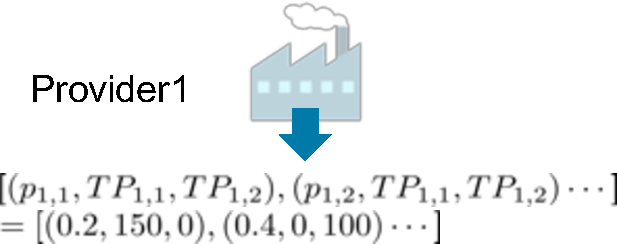
\includegraphics[width=0.2\textwidth]{bid-provider-single.pdf} 
  \caption{Bid of provider in double auction}
  \label{fig:bid-provider-double}
\end{figure} 
リソース要求側($\j=1 \cdots J$)の入札について説明する.
\begin{itemize}
\item {入札$n$,予算$v_{n,j}$要求するリソース$r$の要求時間$TR_{j,n,r}$を提示する} 
\item {各企業は$N$個の入札を作成}
  \begin{itemize}
  \item {ただし勝者となる入札は1つ} 
  \end{itemize}
\item {必要なリソースの組合せに対して入札を作成する}
    \begin{itemize}
    \item {全てのリソースが揃わないと製品の生産が出来ないからである}
    \item {1つの要求内のリソースはある1提供企業によって提供されるとする}
    \end{itemize}
\end{itemize}
リソース要求側の入札($i=1 \cdots r$)は,シングルオークションリソース要求と形式は同じである.しかし
入札の予算が評価値として,配分と取引価格の決定に用いられる点で異なる.
\subsubsection{勝者決定問題}
ダブルオークションに基づく手法の勝者決定問題の定式化を\Eqref{ダブル-目的関数}か
ら\Eqref{ダブル-決定変数}に示す.
\begin{flalign}
  % 目的関数
  {\rm max} \quad &\sum_{j=1}^{J}\sum_{n=1}^{N}v_{j} \times y_{j,n} \nonumber \\
  &-\sum_{i=1}^{I}\sum_{r=1}^{R}\sum_{j=1}^{J}\sum_{n=1}^{N}c_{i,r}\times
  TR_{i,n,r}\times x_{i,r,j,n} \label{ダブル-目的関数} \\
  % 提供側の容量制約
  {\rm s.t.} \quad &\sum_{j=1}^{J}\sum_{n=1}^{N}TR_{j,n,r}  \times x_{i,r,j,n}
  \leq TP_{i,r} \quad (\forall i, \forall r)  \label{ダブル-容量制約} \\
  &\begin{cases}
    x_{i,r,j,n} = 0 &({\rm if} \ y_{j,n}=0)  \\
    \sum_{i=1}^{I}\sum_{n=1}^{N} TR_{j,n,r} \times x_{i,r,j,n}\\
    \quad = TR_{j,n,r}
      &({\rm if} \ y_{j,n}=1) 
  \end{cases}
  \label{ダブル-組合せ制約} \\
  % 要求企業jの入札nのリソースrを提供するのは高々1企業とする制約
  &\sum_{i=1}^{I}x_{i,r,j,n} \leq 1  \quad (\forall r, \forall j , \forall
  n) \label{ダブル-提供者数制約} \\ 
  % 要求企業jの入札のうち勝者となる入札は高々1つとする制約
  &\sum_{n=1}^{N}x_{i,r,j,n} \leq 1 \quad (\forall i, \forall r, \forall
  j) \label{ダブル-入札勝者数制約x} \\ 
  % 要求企業jの入札のうち勝者となる入札は高々1つとする制約
  &\sum_{n=1}^{N}y_{j,n}  \leq 1 \quad (\forall j) \label{ダブル-入札勝者数制約x} \\
  % 要求企業jの予算制約
  &\sum_{i=1}^{I}\sum_{n=1}^{N}\sum_{r=1}^{R}PAY_{i,r,j,n} \leq v_{j,n} \quad
  (\forall j, \forall n) \label{ダブル-予算制約} \\
  % 決定変数
  &x_{i,r,j,n},y_{j,n} \in {0,1} \label{ダブル-決定変数} 
\end{flalign}
\Eqref{ダブル-目的関数}は目的関数であり,総利益最大化とする.ダブルオークションの目的関
数は,提供側,要求側双方の評価値,つまりコストと予算により表現する.この定式化
は,予算が高い入札ほど選ばれ安く,また,コストが低いリソースほど選ばれやす
いものとなっている.制約式である\Eqref{ダブル-組合せ制約}から\Eqref{ダブル-決定変数}は,
シングルオークションの勝者決定問題の定式化と同様である.
\subsubsection{取引価格決定}
取引価格$PAY_{i,r,j,n}$を,参考文献\cite{Parnia}を参考に\Eqref{取引価格}のように定める.
ダブルオークションに基づく手法は取引価格を提供側,要求側の双方の評価値,つまりコ
ストと予算より決定する.\Eqref{取引価格}は,お互いの希望の半分で取引することを示
す.
\begin{flalign}
  PAY_{i,r,j,n} = \frac{c_{i,r} + v_{i,j} \times
    (\frac{TR_{j,n,r}}{sumTR_{j,n}})/TR_{j,n,r}}{2} \times TR_{j,n,r} \label{取引価格} 
\end{flalign}
ここで$sumTR_{j,n}$はリソース要求企業$j$がリソースを要求する時間の合計であり,
\Eqref{合計時間}で求まる.
\begin{flalign}
 sumTR_{j,n} = \sum_{r=1}^{R}TR_{j,n,r} \label{合計時間}
\end{flalign}
\section{計算機実験}
シングルオークションに基づく手法と,ダブルオークションに基づく手法について,計
算機実験を行い総利益,総コストを比較する.リソース提供側の提供時間を7段階で設
定し,特性の評価を行
う.提供時間が 多いほどリソース提供側の余裕時間が増加すること示す.勝者決定問題は最適化ソルバーであるCPLEXで求解する.
\subsection{実験条件}
\begin{itemize}
  \item {リソースの種類$R=4$}
  \item {各試行を5回行う}
  \item{提供企業数$I=10$}
    \begin{itemize}
    \item {各企業2種類のリソースを提供する} 
    \item {$TP_{i,r}$[Ts]は乱数で定める.以下のように乱数の範囲を変化させる

           [50,150],[100,200],[150,250],[200,300],

           [250,350],[300,400],[350,450]}
    \item 
    \item {ダブルオークションのコストは$c_{i,r}=[0.1,0.5]$とする}
    \item {シングルオークションの提供単価は提案手法のコストから利益率が(40\%,
        60\%)となるような値を提示する}
    \item {ペナルティ$\alpha=10000$} 
    \end{itemize}
  \item{要求企業数$J=10$}
    \begin{itemize}
    \item {各企業$N=3$ 個の入札を作成}
    \item {要求時間は$TR_{i,n,r}=[0,200](\forall i, \forall n, \forall r)$[Ts]とする} 
    \item {予算は$v_{j,n}=sumTR_{j,n} \times [1.0,1.5]$とする}
    \end{itemize}
\end{itemize}
\subsection{結果と考察}
Table 1から4に実験結果を示す.\tabref{tab:profit}は総利益を表し,
\tabref{tab:trade}取引価格を表す.\tabref{tab:request_rate}は満たされた要
求の割合を示し,\tabref{tab:provide_rate}は提供率(実際に提供した
時間を提供可能時間で割ったもの)を表す.各Tableの値はそれぞれ5試行の平均と分散を表
している.\par
\tabref{tab:profit}よりダブルオークションの方がどの場合においても総利益は高くなっ
た.また,提供時間が長くなるに連れ,シングルオークションは総利益が上昇しなくなった
が,ダブルオークションは提供時間が長くなっても総利益が上昇していることがわかる.
ダブルオークションの総利益が伸び続けたのは,予算を考慮した配分い,予算が高い入札
ほど選ばれやすくなったからである.行ったからである.これは\tabref{tab:trade}において,提供時間[300,400]辺りまで取引価格
が上昇していることからもわかる.また\tabref{tab:trade}の提供時間[350,450]におい
て取引価格が下がったのは,よりコストの安いリソースの提供時間が増えたからであると
考えられる.ダブルオークションの目的関数が双方の評価値であるコストと予算を考慮した
総利益最大化の配分,そして双方の希望価格の半分が取引価格となっているのでこのような結果となった.それに対し,シングルオークションの総利益が伸びなくなった理由は2つ考えられる.1つ目が\tabref{tab:request_rate}より,
全ての要求が満たされたからである.2つ目が提供側の評価値,提供単価のみで配分を決定するシングルオークションでは予算を考慮できない
ため,より予算が高い要求を満たそうとしなかったからである.また,\tabref{tab:provide_rate}より,提供時間が長くなるに連れて,シ
ングルオークションは提供率が大幅に減少するが,ダブルオークションの提供率の減少は
シングルオークションより緩やかであることからも,ダブルオークションがより予算の高
い入札を勝者とする配分となっていることがわかる.
\begin{table}[H]
  \caption{Profit}
  \centering
  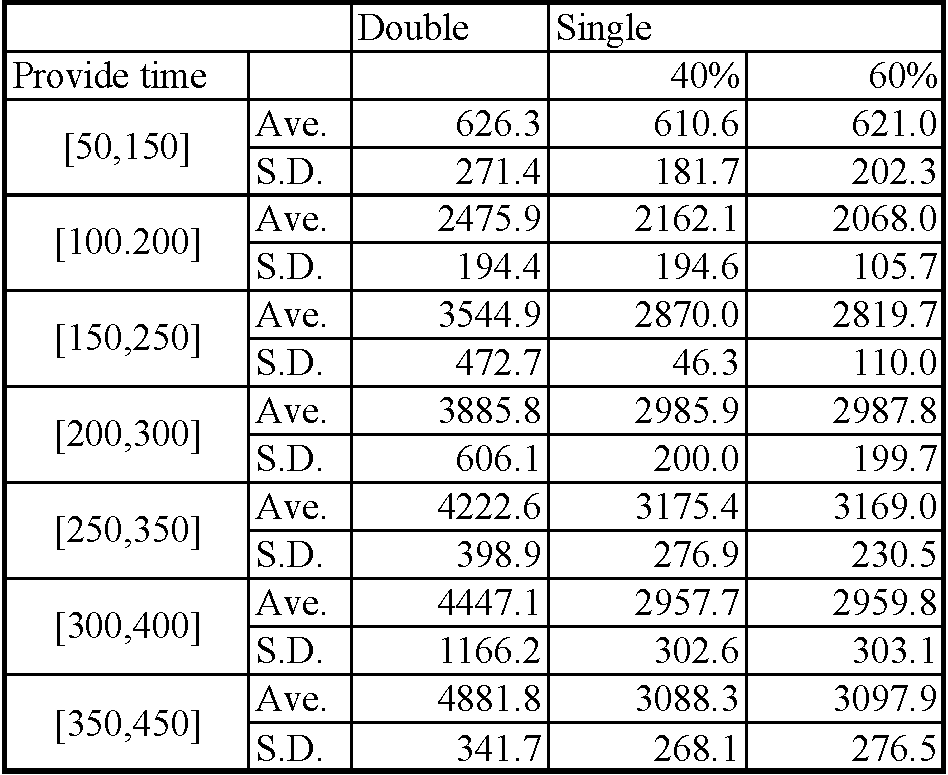
\includegraphics[width=0.4\textwidth]{profit.pdf} 
  \label{tab:profit}
\end{table}

\begin{table}[H]
  \caption{Trade price}
  \centering
  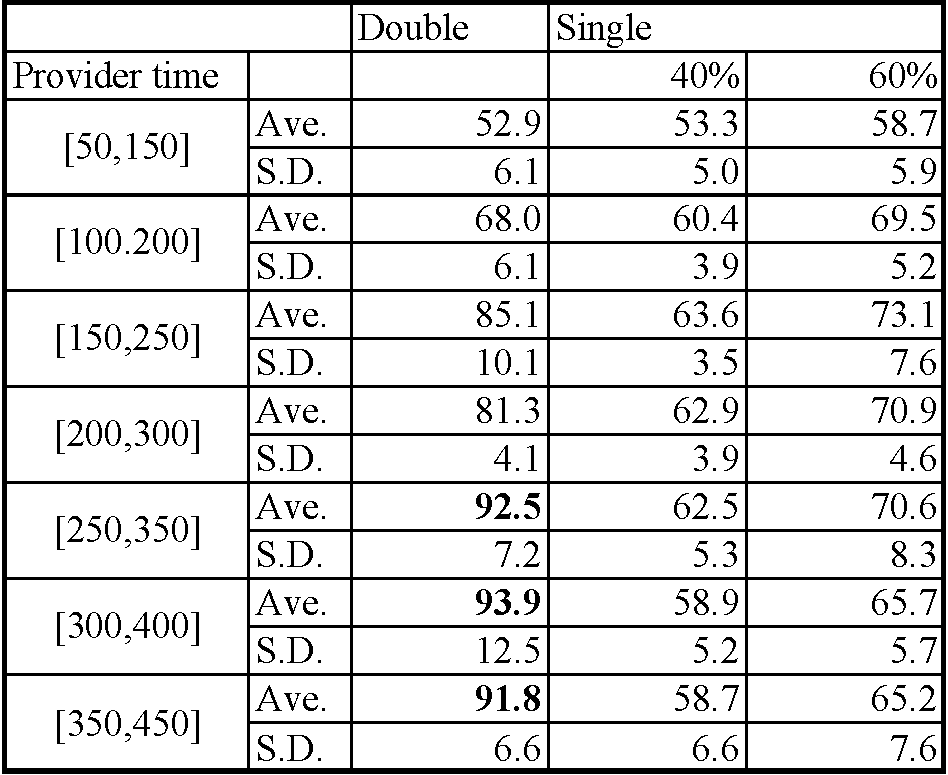
\includegraphics[width=0.4\textwidth]{trade.pdf} 
  \label{tab:trade}
\end{table}

\begin{table}[H]
  \caption{Rate of Satisfied request}
  \centering
  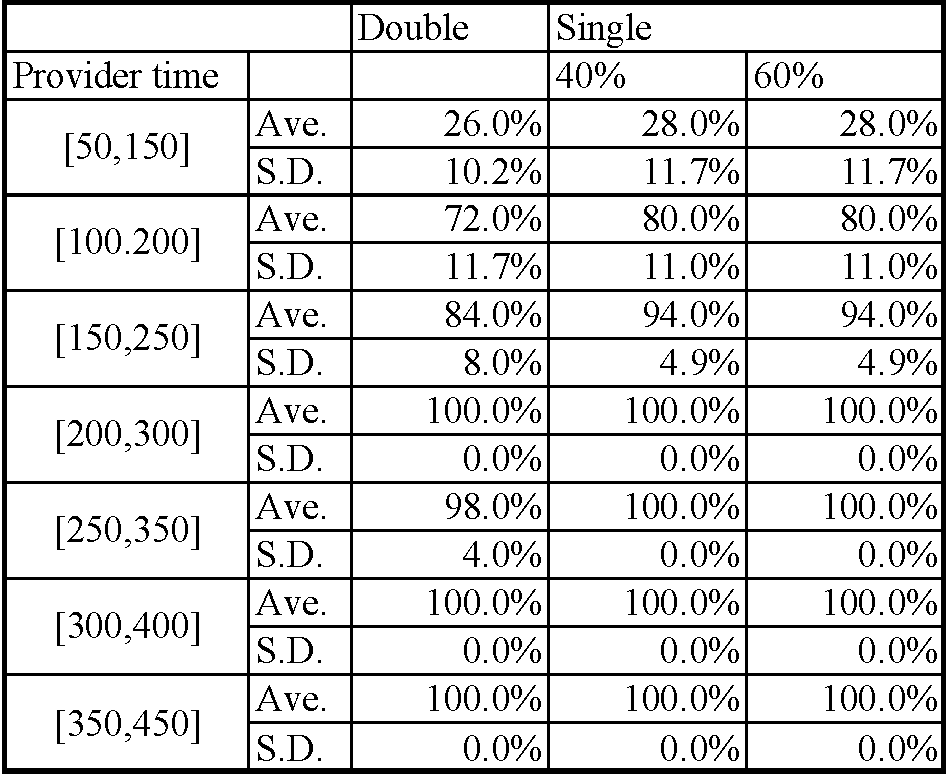
\includegraphics[width=0.4\textwidth]{request_rate.pdf} 
  \label{tab:request_rate}
\end{table}

\begin{table}[H]

  \caption{Rate of resourcec provided}
  \label{tab:provide_rate}
  \centering
  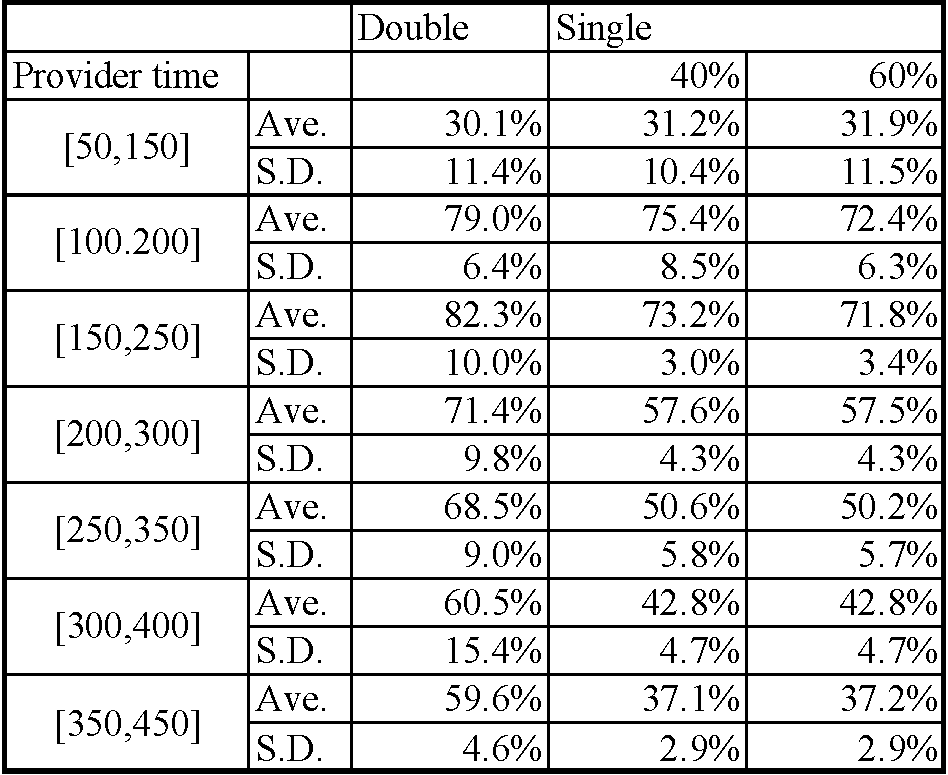
\includegraphics[width=0.4\textwidth]{provide_rate.pdf} 
\end{table}

\section{まとめ}
本稿では,クラウドソースドマニュファクチャリングに対し,シングルオークションに基
づくリソース配分手法とダブルオークションに基づくリソース配分手法の提案,比
較し,特性の評価を行った.得られた結果より,総利益は提供時間を変化させたどの
場合においてもダブルオークションに基づく手法の方が高くなった.構成する企業がそれ
ぞれ独立した企業であるクラウドソースドマニュファクチャリングにおいては,総利益が
高いダブルオークションに基づく手法の方が有効であると考える.\par
今後は,本稿が考慮していない各企業の稼働率の考慮と,オークションにおいて重要とされる耐戦略性を考慮した取引価格決
定方法の提案を行う.
\bibliography{sci} 
\bibliographystyle{junsrt}
\end{document}
% end of sci.tex
